\documentclass[a4paper]{article}
\usepackage[utf8]{inputenc}
%\usepackage[margin=1in]{geometry}
\usepackage{tikz-uml}
\usepackage[tmargin=1in,bmargin=1in,lmargin=1.25in,rmargin=1.25in]{geometry}

% \title{Group of Seven Report}
% \author{1756850 Alkhamra, Othman Bader \\
% 1739256 Benicek, David \\
% 1770922 Bari, Aadam Ali \\
% 1425704 Mankani Vinod, Hitesh \\
% 1755013 Obimma, Timothy Uzochukwu \\ 
% 1783087 Vaddiraju, Nagarjuna}
% \date{January 2018}

\usepackage{natbib}
\usepackage{graphicx}
\usepackage{url}
\usepackage{lipsum}

\usepackage{etoolbox}

% \BeforeBeginEnvironment{figure}{\vskip-2ex}
% \AfterEndEnvironment{figure}{\vskip-1ex}

\newcommand{\subsubsubsection}[1]{\paragraph{#1}\mbox{}\\}
\setcounter{secnumdepth}{4}
\setcounter{tocdepth}{4}

\begin{document}
	\begin{titlepage}
		\newcommand{\HRule}{\rule{\linewidth}{0.5mm}} % Defines a new command for horizontal lines, change thickness here
		\newcommand{\hRule}{\rule{\linewidth}{0.1mm}} % Defines a new command for horizontal lines, change thickness here
		\centering
		
\includegraphics[width=0.2\textwidth]{kcl.png}\par\vspace{1cm}
		\textsc{\LARGE King's College London}\\[1.5cm] % Main heading such as the name of your university/college
		\textsc{\large 7CCSMGPR}\\[0.5cm] % Major heading such as course name
		\textsc{\Large Group Project}\\[0.5cm] % Minor heading such as course title
		\HRule\\[0.4cm]
		{\huge\bfseries Group of Seven Report}\\[0.4cm] % Title of your document
		\HRule\\[1.5cm]
		\vspace{1cm}
		\textit{Authors: }\vspace{0.5cm}
		\begin{center}
			\begin{tabular}{ c|c|c } 
				\hline
				\textbf{Number} & \textbf{Name} & \textbf{Email} \\
				\hline
				1756850 & Othman \textsc{Alkhamra} &  othman.alkhamra@kcl.ac.uk \\ 
				\hline
				1739256 & David \textsc{Benicek} &  david.benicek@kcl.ac.uk \\ 
				\hline
				1770922 & Aadam \textsc{Bari} &  
				aadam.bari@kcl.ac.uk\\ 
				\hline
				1425704 & Hitesh \textsc{Mankani Vinod} &  hitesh.mankani\_vinod@kcl.ac.uk \\ 
				\hline
				1755013 & Timothy \textsc{Obimma} &  timothy.obimma@kcl.ac.uk \\ 
				\hline
				1783087 & Nagarjuna \textsc{Vaddiraju} &  nagarjuna.vaddiraju@kcl.ac.uk \\ 
				
				\hline
			\end{tabular}
		\end{center}
		
		\vfill
		supervised by\par
		Dr.~Laurence \textsc{Tratt}\\
		\vfill
		{\large \today\par}
	\end{titlepage}
	% \maketitle
	\newpage
	\pagenumbering{roman}
	\tableofcontents
	\newpage
	\pagenumbering{arabic}
	\section{Introduction}
	%In this section: Describe the context for the work and the problem you are addressing. Briefly summarise what you achieved in the project.
	
	In real life, we have different objects such as spheres, cubes ... etc. What's mutual between them is that they are all geometry objects. However, those objects might appear in different ways, based on their environment. For example, a mirror sphere placed in an environment with many light sources will react in a different way than a metal sphere. And so, it is clear that different factors such as the material type, light sources and many other factors, will produce many different outputs. \\
	\par Ray tracing is one of the techniques which helps in producing different images for different environment variables. It is widely used in producing films, video games, animations and many other areas. It can be applied on any object and not just geometry objects.
	\subsection{What is the Idea behind  Ray Tracing?}
	Before discussing the idea behind ray tracing, and explaining its algorithm. Let's begin with listing the basic required elements to run the ray tracing algorithm. Those elements will be in one container which will be called \textbf{scene}. The elements of the scene are:
	\begin{itemize}
		\item \textbf{Object(s)}: a scene can contain one or many objects. Each object can be one of the previously mentioned objects types or any other object, which exists in real life. For example, an object could be a sphere, triangle, tree, car, building ... etc.
		\item \textbf{Light source(s)}: The algorithm of ray tracing itself doesn't require having a light source. However, a scene without any light source isn't very practical for ray tracing.
		\item \textbf{Image Plane}: referred to as \textbf{window frame} in our implementation. This plane has a set width and height and it is divided into small squares, where each square covers a number of pixels on the objects of the scene.
		\item \textbf{Eye or Camera:} In order to render the scene, it is mandatory to have an eye or camera, with a certain position and direction. The camera is used to determine the way of looking to the scene elements. From the eye or camera, view rays are produced which travel through the image plane and determine the way the object is rendered.
		%DB-NOTE: I change the last bullet point - let's just double check this is correct
		
		%DB-NOTE: The top part is a good intro, I think bellow is getting a bit too technical for introduction. In the end I don't think it matters where we have this info as long as we don't duplicate it here and in the implementation. So this is something we can talk about
	\end{itemize}
	\begin{figure}[ht!]
		\centering
		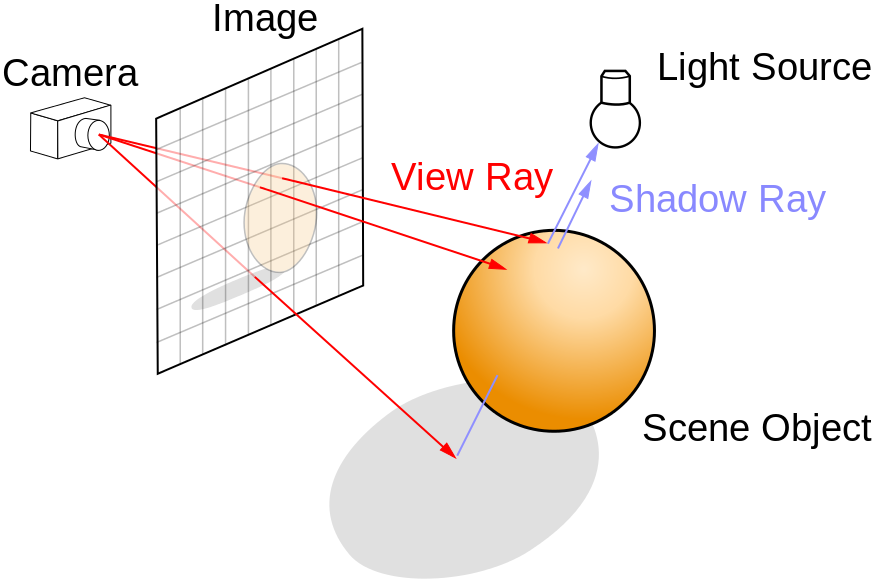
\includegraphics[scale=0.30]{./raytracing.png}
		\caption{Ray Tracing's Scene Elements \cite{raytracingpic}}
		\label{fig:raytracing}
	\end{figure}
	\par \textbf{Figure \ref{fig:raytracing}} shows an example of a scene with the previously listed elements. Now, and after discussing the elements of the scene, it is the time to describe the algorithm of ray tracing. Despite the implementation not being trivial, the main idea is quite simple; in each scene there will an eye or camera, from that camera many rays will be produced and go across the small squares in the image plane, for each ray we need to check whether it intersects with any of the objects or not, and return the colour of that pixel. Other rays are possible to be produced caused by reflection. These rays also will follow the ray tracing algorithm before returning the final colour.\\
	\par The algorithm itself is really simple. Nevertheless, it is previously mentioned that environment variables play a big role in the calculations. And so, returning the colour of the pixel, which was hit by the the ray, won't be that simple; since it will require additional computations related to the reflections, shades ... etc. 
	\subsection{Our Solution}
	Although the idea behind ray tracing is simple, there are many different problems to be addressed in this program. These problems can be summarised as below:
	\subsubsection{Web Interface}
	In order to define the different elements of the scene, a web interface is developed to allow users enter the different values for the scene elements. Using this interface, the user can add different objects to the scene, with different materials, positions, sizes, colours. Furthermore, adding different lights at different positions with different colours. \\
	\par The challenge here is that objects must be in 3D. And so, we developed a web interface with two options. One option is the 2D option, where the user needs to define an element by providing its values in the top and side views. The other option, is the 3D view, where the user can add elements directly in 3D format.\\
	\par All the functionality in our 2D web interface supports the drag and drop feature. In other words, the user can define the position by clicking on the object, moving it in any direction, and from the 3D view, the user can view the scene.
	%DB-NOTE: Is this true? We don't have drag and drop in 3D
	\subsubsection{Ray tracing Engine}
	The other part of our system is the back-end engine, where all the calculations are done based on the input received from the web interface. This system was developed using .NET C\#. It includes a post API, which will receive the request from the client, and it is able to render a scene with the following:
	\begin{itemize}
		\item A scene with the following objects:
		\begin{itemize}
			\item \textbf{Plane}: This object is mainly used to create the walls in the scene. And it has a position, and a vector called normal which decides the orientation, in addition to one of the supported materials.
			%DB-NOTE: A normal what?
			\item \textbf{Cube}: Each cube has a size, a position, and is made up of one of the supported materials.
			\item \textbf{Sphere}: Each sphere has a radius, centre point, and is made up of one of the supported materials.
		\end{itemize}
		The  \textbf{supported materials} are:
		\begin{itemize}
			\item \textbf{Phong materials}:  which follows the phong theory such as chalk, metal, plastic. The difference between those materials is the values of diffusion, specular coefficients and the light colour influence.
			\item \textbf{Flat material}: which is the simplest material, that will return the colour of that object regardless to any other environment variables and parameters.
			\item \textbf {Mirror material}: this material is the most complicated one, which will do many different calculations in order to calculate the colour of each pixel of that object.
			%DB-NOTE:  This is reflective right? Might want to add that in
		\end{itemize}
		Each of these materials can have a colour chosen by the user, or just use the default colour, if null.
		%DB-NOTE: can we say null here instead?
		\item A scene with multiple light sources at different positions and colours.
		\item A scene with perspective camera. Each camera has a position, direction of how to look at the image plane, and distance from that plane.
	\end{itemize}
	\section{Review}
	\subsection{Brief History of Ray tracing}
	
	\par Ray tracing is one of the popular methods of rendering. What is Rendering? Rendering is the act of generating an image (usually photorealistic) from a 2D or 3D model. There are three familiar techniques to image rendering and they are rasterisation, ray casting and ray tracing. These three techniques are quite similar but are differentiated by their representation of the optical effects such as reflection intensity which in turn makes the processing speed vary differently (Wald, Slusallek, Benthin, \& Wagner, 2001). This means that ray tracing would produce the most photorealistic image while also taking the most time to compute while rasterisation would produce the most basic image.\\
	
	\par The earliest known Ray tracing system was calculated by hand by Richard Hoyt in the 1950's while working on vehicle shotline at the Ballistic Research Library known today as DARPA (Klopcic \& L. Reed, 1999). In the 1960's, physicists coined the name "ray tracing" by plotting on paper the path taken by rays of light starting at a light source and passing through the lens in the design of lenses (Glassner, 1989).\\
	
	\par Computer Graphic researchers at the university of Utah thought it would be a good idea to apply this simulation of light physics to create images but the computers of the 1960's were too slow to produce images of better quality than those made by using cheaper image rendering techniques hence the idea of ray tracing was dropped for several years.\\
	
	\par Over several years, as computers grew more powerful, it became imperative to simulate the real physics. Several optimised algorithms were implemented and this led to computers being able to simulate various kinds of optical effects. Ray tracing have evolved greatly since then and is now one of the most powerful technique used in image rendering. Ray tracers have become both faster and more efficient and can even produce hyper-realistic images that are indistinguishable from the real world. We will Discuss some Ray tracers in 2.3.\\
	
	\subsection{Overview of Ray Tracing}
	\par Ray tracing is a simple and powerful technique. It involves shooting rays from a point-of-view (usually represented by an eye or a camera). These rays then go through each pixel of the viewing plane and some calculations are done to determine if they intersect with objects. When an intersection is detected, reflected or refracted rays are always generated (Weghorst, Hooper, \& Greenberg, 1984). Each of the reflected/refracted rays must be recursively calculated to determine which surfaces they intersect. At each pixel where intersection occurs, the ray tracer must work out the intensity of the light and how much of it reflected back in order to determine the exact colour of the pixel (Suffern, 2007). This is usually a long process and the time taken to generate each image increases exponentially with respect to an increase in the size of the viewing plane(image frame).\\
	
	\subsection{Review of Related Works}
	\par In this section, the Ray tracers discussed either helped influence our design decisions or have a similar structure to what we have built.
	\subsubsection{Ray Tracing from the Ground Up}
	\par This is a book written by Kevin Suffern.
	
	\subsubsection{BRL-CAD}
	\subsubsection{OpenRL}
	%DB-NOTE: this sounds dope! Are Nvidia Optix,BRL-CAD and OpenRL all thing we used or considered using?
	
	\section{Requirements and design}
	
	%In this section: Describe the requirements you set for your project at the beginning and the design you have taken for your project. Focus on why you decided to tackle the problem in the way you did, and what effects that had on the design. You may also wish to mention the impact of team-working on your requirements and design.
	
	\subsection{Mandatory Requirements}
	
	
	The beginning of the project saw the group discuss and decide what features were essential for the running of the ray tracer, that is to say, creating and developing a running system, consisting of the front-end, which is the client side, and the back-end, which is the server side. The bare minimum requirements for the entire system are as follows:
	\begin{itemize}
		\item Allow users to create spheres and cubes with specific parameters' values. Those parameters are:
		\begin{itemize}
			\item The size of the object.
			\item The position of the object.
			\item The material of the object; determining its colour and translucency.
		\end{itemize}
		\item Allow users to assign values to the parameters of the environment. The parameters include the following:
		\begin{itemize}
			\item Position of the camera.
			\item Size of the output image and the window frame.
			\item Filename of the output image.
			\item Colour of the background.
			\item Light's colour and position.
		\end{itemize}
		\item Render multiple objects in the same scene, with at most one light source.
	\end{itemize}
	
	
	\subsection{Optional Requirements}
	
	If time allowed, the group established additional requirements.
	The requirements specified in this category will extend the basic functionality of the raytracer, thus distinguishing our product from others. The optional requirements are as follows:
	\begin{itemize}
		\item Allow users to add multiple lights to the scene in different positions, colours and intensities.
		\item Allow users to create other objects such as polygons.
		\item Allow users to choose different materials, such as plastic, mirror, etc. for the objects.
		\item Improve the colours of the output image, by using different techniques such as sampling.
		\item Improve the performance of our system, by applying the multithreading concept, if the systems takes a long time while rendering the scene.
	\end{itemize}
	
	Due to time constraints we were unable to implement the use of polygons. However we successfully achieved the other optional requirements. 
	
	
	\subsection{Methodology}
	
	The methodology the group decided to adopt was the Agile software methodology. 
	
	\subsection{Architecture}
	
	
	This project has a two-tier, client-server architecture.
	
	1.  The front-end client is served up by the server.  The front-end has a user interface that allows the user to input their shapes and it will also dynamically render an approximation of the input to visualise what the user is about to ray trace.  The front-end will primarily be coded in HTML, CSS, JavaScript and AJAX.
	
	%OK-NOTE: It is just one controller.
	2.   The  back-end  has  a  number  of  controllers  that  will  dynamically  process  the content specified by the user and generate a ray traced image.  The back-end is built in .Net, using WebApi2 to run the local server.
	
	\subsection{Architectural Pattern}
	
	As we were using ASP.NET, it only made sense for the group to take advantage of the ASP.NET MVC web application framework. This framework implements the model–view–controller (MVC) pattern and allowed us to divide the application into a composition of three main logical components: Model, View and Controller. 
	
	\begin{figure}[ht!]
		\centering
		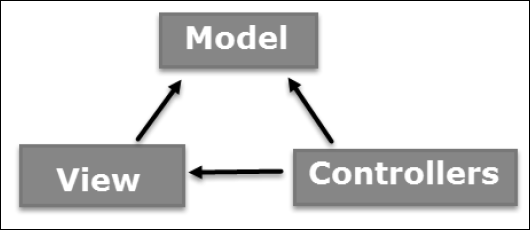
\includegraphics[scale=0.70]{./model_view_controller.jpg}
		\caption{Components of MVC}
		\label{fig:mvc}
	\end{figure}
	
	\begin{itemize}
		\item \textbf{Model} - 
		\item \textbf{View} - 
		\item \textbf{Controller} - 
	\end{itemize}
	
	
	\subsection{Prototypes}
	
	\section{Implementation}
	
	%In this section: Describe the most significant implementation details, focussing on those where unusual or detailed solutions were required. Quote code fragments where necessary, but remember that the examiners have full access to your source code. Explain how you tested your software (e.g. unit testing) and the extent to which you tested it. If relevant to your project, explain performance issues and how you tackled them.
	
	\subsection{Front End}
	\subsection{Back-end}
	As mentioned before, the ray tracing algorithm is mainly about checking if the ray, which goes from the camera or reflects from objects because of lights, hits/intersects with the object or not. Furthermore, ray tracing depends on the material of each object, and so we should take that into our consideration. In addition to that, each scene has lights and cameras, and since each of these can have different type, we need to implement that to be scalable and open for extension.\\
	\par In our implementation we make use of different object oriented principles such as abstract classes, inheritance, overriding and Polymorphism. In the following sections, we will discuss in details how we used each of these concepts in our codes.
	\subsubsection{Basic Elements}
	There are many basic elements which are required to build a ray tracer. These elements were reflected in our project as classes: 
	\begin{itemize}
		\item \textbf{Point3D}: This class is used to create a point in the 3D with x,y and z double values. In this class all the addition, subtraction, division and multiplication were overridden in order to perform them correctly in the context of points. Also, there are other methods such as the distance, which will be used to return the distance between two points.
		\item \textbf{Vector3D}: This class is used to create a vector in the 3D with x,y and z double values. In this class all the addition, subtraction, division and multiplication were overridden in order to perform them correctly in the context of vectors. Also, there are other methods such as the length, which will be used to return the length of a vector. Furthermore, the dot and cross products methods were implemented; since they are crucial in our project.
		\item \textbf{ColorRGB}: This class is used to create a colour with R, G, and B double values. In this class all the addition, subtraction, division and multiplication were overridden in order to perform them correctly in the context of colours.
		\item \textbf{Point2D}: This class is used to create a point in 2D with x and y double values. No other methods were added to this class; since they are not needed in this class.
		\item \textbf{Ray}: This class is used to create a ray, which will have an origin with type of \textbf{Point3D}, and a direction with type of \textbf{Vector3D}. This ray will be used in most of the calculations of ray tracing. There are no methods directly implemented in this class, but it will make use of other methods implemented in \textbf{Point3D} and \textbf{Vector3D}.
	\end{itemize}
	\subsubsection{Configurations}
	In order to make it easier to change any configured value in our program, we created a class called \textbf{Config}, where you can find any default values used in our program. By doing that, we make sure that changing the value in one place will change it in all the places where it is used. For example, the default colour, material, vector, point ... etc are defined in that class. 
	\subsubsection{Materials}
	One of the main factors which will affect the final result of ray tracing is the material of the object. All materials will have a colour, in addition to many different coefficients that might be needed for other materials, such as the diffusion, specular, ambient. In each material, we need a method that will calculate the shades caused by lights and other objects. \\
	\par It is clear that we need to have an abstract class with the previously mentioned attributes, in addition to an abstract method which will be called calculateShade, which will be implemented differently based on the material. As we mentioned in the introduction, we covered three types of materials. The class diagram for this part of our program is shown in Figure \ref{fig:matcd}.
	\begin{figure}[ht!]
		\centering
		%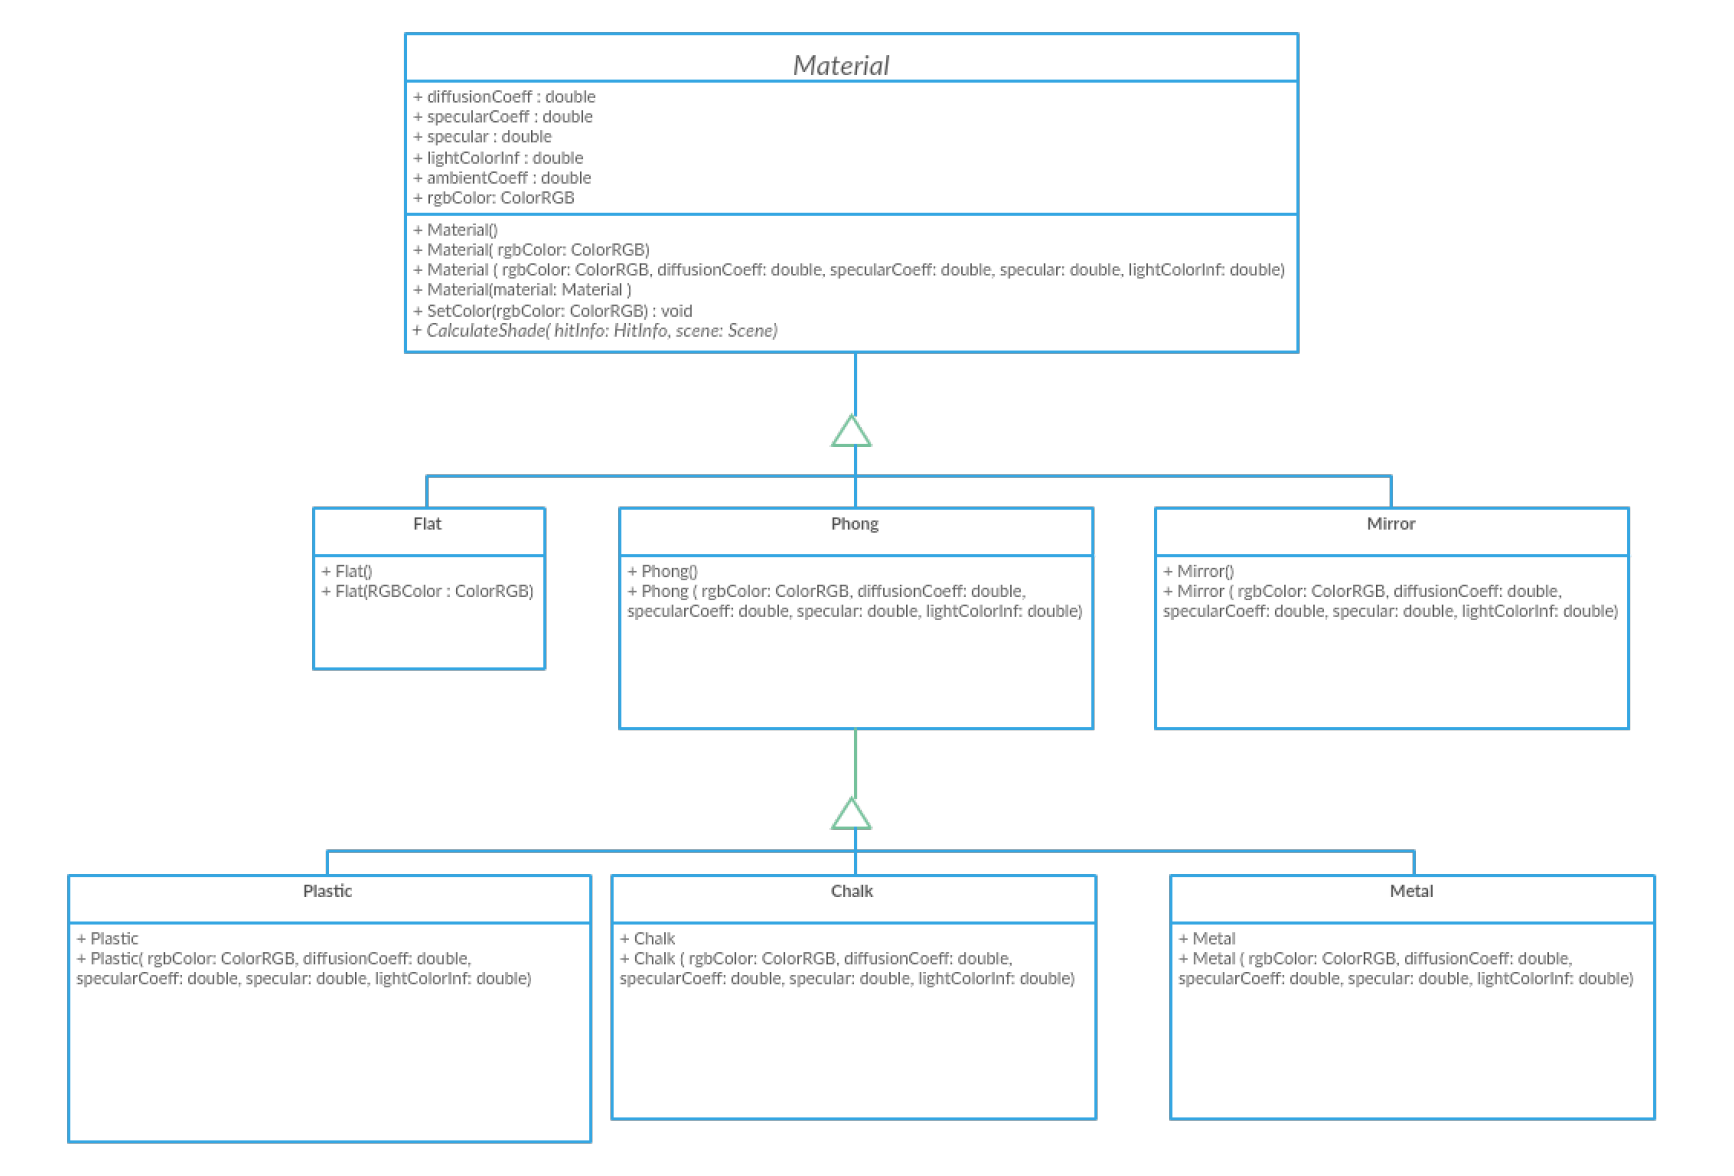
\includegraphics[scale=0.50]{./materials.png}
		\begin{tikzpicture}[scale=0.8, every node/.style={scale=0.8}]
		\umlclass[type=abstract]
		{Material}
		{
			+ diffusionCoeff : double\\
			+ specularCoeff : double\\
			+ specular : double\\
			+ lightColorInf : double\\
			+ ambientCoeff : double\\
			+ rgbColor: ColorRGB
		}
		{
			+ Material() \\
			+ Material( rgbColor: ColorRGB) \\
			+ Material ( rgbColor: ColorRGB, diffusionCoeff: double, \\ \hspace{0.15cm} specularCoeff: double, specular: double, lightColorInf: double)\\
			+ Material(material: Material )\\
			+ SetColor(rgbColor: ColorRGB) : void\\
			+\umlvirt
			{CalculateShade (hitInfo: HitInfo, scene: Scene = null ): HitInfo 
			} 
		} 
		\umlclass[x=0, y=-7]{Phong}{}
		{
			+ Phong ()\\
			+ Phong  ( rgbColor: ColorRGB,  \\ \hspace{0.15cm} diffusionCoeff: double, \\ \hspace{0.15cm} specularCoeff: double,  \\ \hspace{0.15cm} specular: double, \\ \hspace{0.15cm} lightColorInf: double)\\
		}
		\umlclass[x=7.2, y=-7]{Flat}{}
		{
			+ Flat() \\ 
			+ Flat(RGBColor : ColorRGB)
		} 
		\umlclass[x=-7.2, y=-7]{Mirror}{}
		{
			+ Mirror () \\
			+ Mirror ( \\  \hspace{0.15cm} rgbColor: ColorRGB = WHITE,  \\ \hspace{0.15cm} diffusionCoeff: double = 1.0, \\ \hspace{0.15cm} specularCoeff: double = 0.5 ,  \\ \hspace{0.15cm} specular: double = 1.0, \\ \hspace{0.15cm} lightColorInf: double = 0.01)\\
		}
		\umlclass[x=-7, y=-12]{Chalk}{}
		{
			+ Mirror () \\
			+ Mirror ( \\  \hspace{0.15cm} rgbColor: ColorRGB,  \\ \hspace{0.15cm} diffusionCoeff: double = 0.4, \\ \hspace{0.15cm} specularCoeff: double = 0.2 ,  \\ \hspace{0.15cm} specular: double = 2.0, \\ \hspace{0.15cm} lightColorInf: double = 0.25)\\
		}
		\umlclass[x=0, y=-12]{Plastic}{}
		{
			+ Mirror () \\
			+ Mirror ( \\  \hspace{0.15cm} rgbColor: ColorRGB, \\ \hspace{0.15cm} diffusionCoeff: double = 0.4, \\ \hspace{0.15cm} specularCoeff: double = 0.2 ,  \\ \hspace{0.15cm} specular: double = 20, \\ \hspace{0.15cm} lightColorInf: double = 0.35)\\
		}
		\umlclass[x=7, y=-12]{Metal}{}
		{
			+ Mirror () \\
			+ Mirror ( \\  \hspace{0.15cm} rgbColor: ColorRGB, \\ \hspace{0.15cm} diffusionCoeff: double = 0.4 \\ \hspace{0.15cm} specularCoeff: double = 0.2 ,  \\ \hspace{0.15cm} specular: double = 100, \\ \hspace{0.15cm} lightColorInf: double = 0.001)\\
		}
		\umlVHVinherit{Phong}{Material} 
		\umlVHVinherit{Flat}{Material} 
		\umlVHVinherit{Mirror}{Material} 
		\umlVHVinherit{Chalk}{Phong} 
		\umlVHVinherit{Plastic}{Phong} 
		\umlVHVinherit{Metal}{Phong} 
		\end{tikzpicture}
		\caption{Materials Class Diagram}
		\label{fig:matcd}
	\end{figure}
	%I need to add a class diagram for this part also.
	\subsubsection{Geometry Objects}
	\label{sssec:geo}
	From the basic idea of ray tracing, we need a method to test whether a ray intersects with the object or not, and since we need our program to be scalable and open for extension, we created an abstract class called geometry object, which will have an attribute called the material; because each object will have a material. In addition to an abstract method called intersect. \\
	\par In order to add a new geometry object, we need to add a new class, which inherits the GeometryObject abstract class. Then add the attributes needed for the new class, and finally implement the intersect abstract method. The intersect returns an object of type \textbf{HitInfo} which will include the following attributes:
	\begin{itemize}
		\item \textbf{hasHit}: boolean attribute which be \textbf{true} if the ray hits the object, and \textbf{false} if not.
		\item \textbf{hitPoint}: it will be the point of where the ray hit the object. This value will be \textbf{ignored}, if \textbf{hasHit} is \textbf{false}.
		\item \textbf{normalAtHit}: it will be the vector which is perpendicular to the hitPoint. This value will be \textbf{ignored}, if \textbf{hasHit} is \textbf{false}.
		\item \textbf{Ray}: it will be the ray which hits the object. This value will be \textbf{ignored}, if \textbf{hasHit} is \textbf{false}.
		\item \textbf{hitObject}: it will be the object which was hit by the ray. This value will be \textbf{ignored}, if \textbf{hasHit} is \textbf{false}.
		\item \textbf{tMin}: it will be smallest value, which is greater than some epsilon value, from many different possible values, that will be produced when a ray hits an object. It will be used to calculate the \textbf{hitPoint}, and it will be \textbf{ignored}, if \textbf{hasHit} is \textbf{false}.
	\end{itemize}
	%I need to add a class diagram for this part
	\par In our program, we have three different objects: \textbf{Sphere}, \textbf{Cube} and \textbf{Plane}. The class diagram for this part of our program is shown in Figure \ref{fig:geo}.
	\begin{figure}[ht!]
		\centering
		%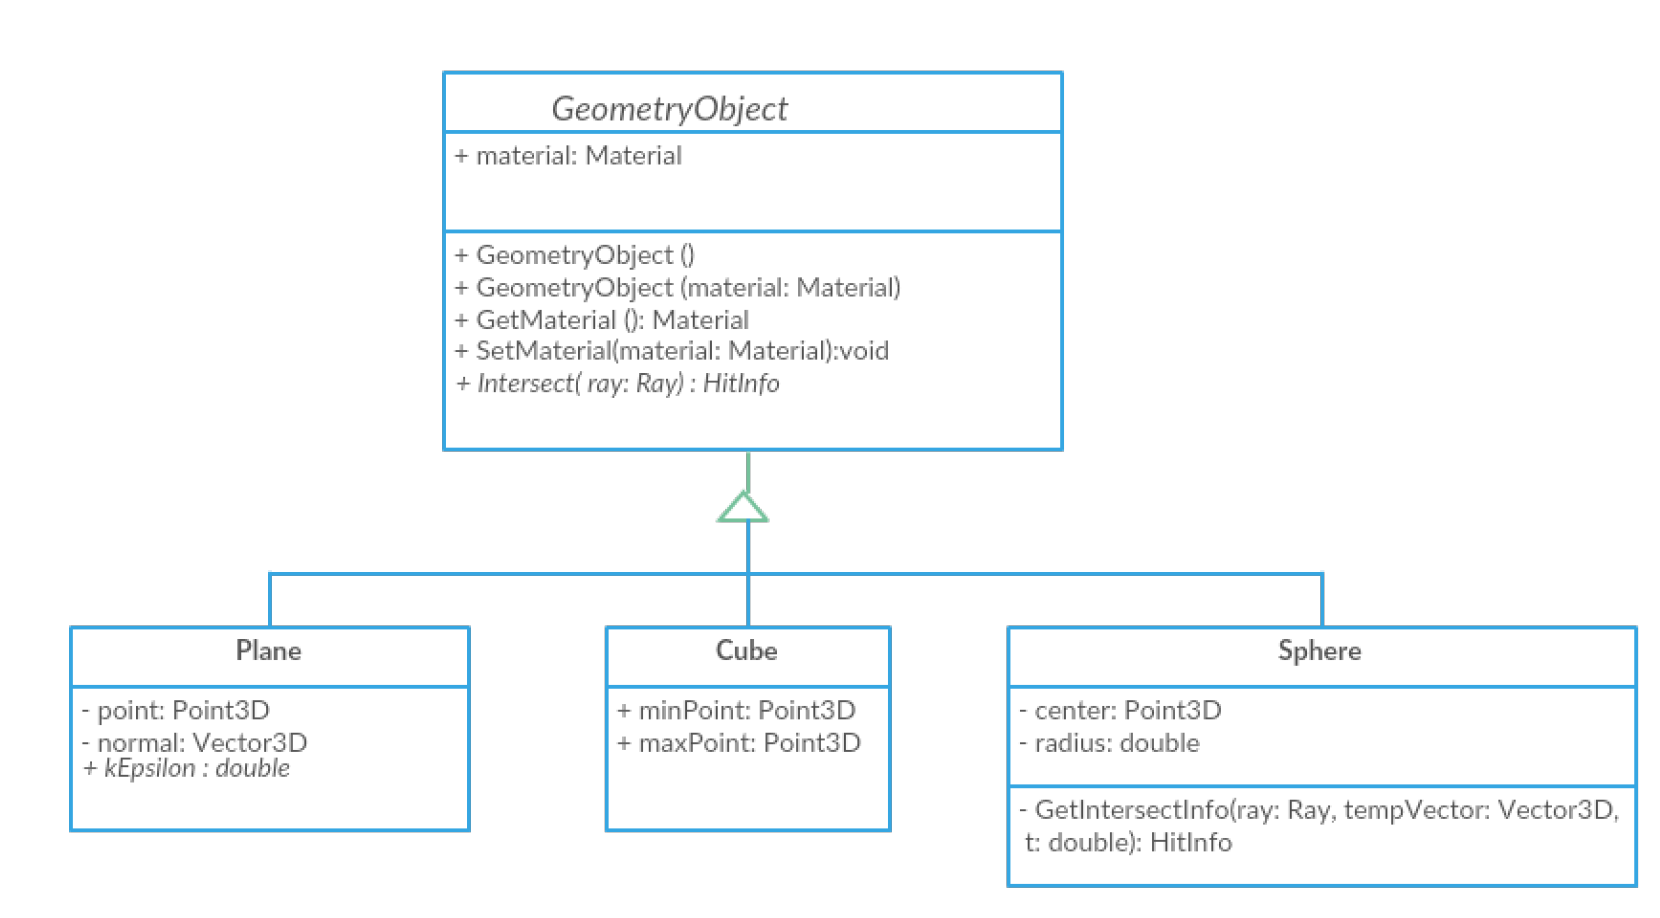
\includegraphics[scale=0.50]{./objects.png}
		\begin{tikzpicture} 
		\umlclass[type=abstract]
		{GeometryObject}
		{+ material : Material}
		{
			+ GeometryObject () \\ 
			+ GeometryObject (material: Material) \\ 
			+ GetMaterial (): Material \\ 
			+ SetMaterial (material: Material): void \\ 
			+ \umlvirt{Intersect (ray: Ray): HitInfo } 
		} 
		\umlclass[x=0, y=-5]{Sphere}
		{ - center: Point3D \\ - radius: double} 
		{
			- GetIntersectInfo(ray: Ray, \\ tempVector: Vector3D, t: double): HitInfo 
		}
		\umlclass[x=6, y=-5]{Cube}{+ minPoint: Point3D \\ + maxPoint: Point3D}{} 
		\umlclass[x=-6, y=-5]{Plane}{
			- point: Point3D \\ 
			- normal: Vector3D \\ 
			+ \textit{kEpsilon : double} 
		}{} 
		\umlVHVinherit{Sphere}{GeometryObject} 
		\umlVHVinherit{Cube}{GeometryObject} 
		\umlVHVinherit{Plane}{GeometryObject} 
		\end{tikzpicture}
		\caption{Geometry Objects Class Diagram}
		\label{fig:geo}
	\end{figure}
	\subsubsection{Lights}
	Each light will have a colour, intensity and a position. There might be different types of lights, and that's why we created a class called \textbf{Light}, and it is not an abstract class; since we want to create instances of it. Therefore, we defined it is method to be virtual, and so they can be overridden if we need to change their default implementation.
	\par The methods in this class are:
	\begin{itemize}
		\item \textbf{GetDistance}: this method will calculate the distance between some point, and the position of the light.	 	\item \textbf{GetDirection}: this method will calculate the direction of the light with respect to some given point.
		\item \textbf{GetColor}: this method will calculate the final colour after considering the light effects, such as the colour and intensity.
	\end{itemize}
	\subsubsection{Tracer}
	The tracer class will be responsible for tracing an input ray with all objects in the scene. Then, if the ray hits one of the objects, it will call the method another time recursively for some predefined depth value. Then, it will use the hitInfo in order to call the \textbf{CalculateShade} method, which was previously discussed in the materials section, and the \textbf{TraceShadeRay} method, which will calculate the effects of lights on the object.\\  
	\par Finally, the result will be the multiplication of the values returned by the previous two methods in case the ray hits one of the objects, otherwise, it will be the colour of the scene's background.
	\subsubsection{Camera}
	\label{sssec:cam}
	Another important element of ray tracing is the camera, which represents the way of looking to the objects in the scene. There are many different types of cameras that can be used such as perspective and orthographic cameras. In our implementation, we used the perspective camera. But in order to keep our program open for any future extension, we created an abstract class called camera, which contains:
	\begin{itemize}
		\item \textbf{Attributes}:
		\begin{itemize} 
			\item \textbf{Position}: which is a 3D point represents the position of the camera in the scene.
			\item \textbf{lookAt}: which is a 3D vector represents the direction of how to look at the scene.
		\end{itemize}
		\item \textbf{Methods and Operations}: These methods will be implemented differently based on the type of the camera
		\begin{itemize} 
			\item \textbf{Render()}: this method will be doing the ray tracing algorithm, by going through all pixels in the window frame and get the colour of that pixel.
			\item \textbf{FindRayDirection(Point2D point)} : this method will calculate the ray direction from a given point in the window frame with respect to the camera's values.
		\end{itemize}
	\end{itemize}
	\par In the perspective camera's implementation, the \textbf{Render} loops through all pixels in the image plane,  and then calculate the point, which in order will be used as an input to \textbf{FindRayDirection} method, and then call the \textbf{TraceRay}, which was discussed before in the previous section. To make the resulting colour smoother, we used one of the sampling techniques called the regular sampling technique.
	\subsubsection{Sampling}
	One of the enhancements that we did to our output is to use one of the sampling techniques. In our application, we used the \textbf{Regular Sampling Technique}. The main idea behind it is to do the tracing on the same square of the image plane, but at different sampling values, and calculate the colour at different points inside that square for \textbf{N \footnote{The number of samples}} times.\\
	\par Finally, we sum up these values together, and divide the result by \textbf{N} which will be the final colour of that square. By applying this technique, the final colour will be smoother than not using any sampling technique at all.
	\subsubsection{Scene}
	The scene will be the container of all the previously mentioned classes. Each scene will have a list of geometry objects, list of lights, camera, background colour, sampler, file name which will be the final name of the output file.\\
	\par The scene will also have many different methods:
	\begin{itemize}
		\item \textbf{GetHitInfo}: This method will find if the ray hits any of the objects in the scene, and will return the hitInfo of the nearest object which was hit by the ray, in addition to other values of hitInfo, which were discussed before in \textbf{Section \ref{sssec:geo}}.
		\item \textbf{Render}: it will call the render method of the camera's object. More details about this method can be found in \textbf{Section \ref{sssec:cam}}.
		\item \textbf{DisplayPixel}: it will take the x and y indices of a point, with the calculated colour as inputs, and then assign that colour to the appropriate index in the final picture pixels result.
		\item \textbf{FinalPicture}: this method will just print the colours in the final pixels array, which are filled by the \textbf{DisplayPixel}, that is called by the \textbf{Render} method, into an image of jpg type, with the filename received from the front end.
	\end{itemize}
	\subsubsection{Api Controller}
	In our project, we have one controller that will act as a post API. It will receive a JSON from the front-end side, the responsibility of that controller is to parse the received JSON, in a way that can be understood by the back-end's implementation. That's why we are having JSON folder in our project.\\
	\par After parsing the JSON, we can create the scene object, then call the  \textbf{Render} method, after that call the \textbf{FinalPicture} method, and finally return the image to front-end.
	\subsubsection{Unit Testing}
	\section{Team work} 
	
	%In this section: Describe how you worked together, including the tools and processes you used to facilitate group work.
	
	\subsection{Process}
	Weekly meetings
	At the start of each meeting standup style sync up:
	Everyone speaks, says what they did, what still needs to be done, calls out any blockers that we can go over in the follow on meeting.
	Discussion: 
	Talk about what the next steps are, what could be improved, what has blocked us in the previous sprint. Try arrive at outcomes - outcomes made into tickets
	Next steps:
	Illicit next steps both from discussion and from product roadmap
	
	
	\subsection{Communication}
	
	Communication is one of the most important factors when it comes to working in a software engineering team. For our project we decided to utilise a number of different structured and unstructured communication channels. There exists a large array of great project management and issue tracking tools such as JIRA, Trac or Trello, however, we decided that given the brevity of our project and the relative low number of backlog items (especially at the start), that it would be best to keep our ticket system as close to the codebase as possible. As a result of this, we decided to make use of the inbuilt GitHub issue tracking system. This system does not provide the same calibre of project management tools as some of the forementioned products, however, it does enough for our purposes. We decided to use the GitHub milestone system as a way of scheduling issues for our sprints and implemented a branch naming convention such that we would refer to the issue we're addressing in the name of the branch - \{issue number\}/\{name of branch\}. This simple mechanism has worked tremendously because it ensures that on one hand all branches are addressing exactly one tasks or feature and on the other hand, that all tasks and features have been recorded in an issue. 
	
	Another way we structured our communication was by the use of pull requests whenever pushing code to master. By raising a pull request and having another team member review it we not only improved our code quality but also spread knowledge of the code base and cross-polinated ideas for features or more efficient solutions. Standout examples of a pull request flow can be seen here: TODO: Cite some nice PR from github
	
	Not all communication can be done over issue summaries and pull requests and therefore we scheduled weekly meetings to go over what has been achieved, what needs to be discussed and what is the plan for the following sprint. One could say that we condensed our daily scrum meeting, sprint planning, backlog refinement and sprint review all into one weekly meeting. This is not the textbook way of running an Agile project but given that we are not working on the project full time and that these meetings were kept as brief as possible, it still alligns to the core principles of Agile. During the meetings we would discuss the general trajectory of the project and what we want to accomplish in the next seven days, before breaking off into our sub teams and deciding on the exact issues we needed to create for the week ahead. This way of running a project has both advantages and disadvantages which is covered in section TODO: Cite section that covers this. We mostly met in person but on occasion, when we needed to, we used video conferencing tools such as Appear.In and Gruveo to connect with eachother.
	
	During the course of the sprints, our communication did not fade. We built on some ideas from Extreme Programming and met frequently in our work units to engage in pair programming while working on issues during the sprint. To facilitate the smooth operation of the team we used the lowest friction medium of communication for all of us which was a WhatApp group where we have discussed everything from meeting times, status of different issues or even specific lines of code in pull request. 
	
	\subsection{Tools}
	
	Things that enabled us
	Visual Studio, Visual Studio Code, Git,
	Things that kept us on track
	Travis, Mocha, Istanbull,
	Things that connected us
	Appear.In, Gruveo, Whatsapp, Facebook,
	
	
	\section{Evaluation}
	Considering the mandatory requirements that were previously set out, all of them have been accomplished. %TODO: double check
	On the other hand, our optional requirements have not been completed. However, if the deadline was not a factor, they would have been completed as most of them were quite similar to the mandatory ones. 
	
	As mentioned earlier, the team was divided into two. This was a success as each team member decided whether they wanted to work in either the front-end or the back-end depending on their own skills,desires or work experience. This was crucial as everyone choose the area they were more comfortable working with which allowed less issues to arise in the future. Each sub-team also had at least one member who had work experience in the particular field. David had experience in the front-end, whereas Othman had experience in the back-end. This was important as both of them were able to lead their sub-team and any problems would be solved efficiently. It also gave the rest of the team members a look into the future as both of their experience helped the team visualise and learn how different code practices and tools are used in the workplace.
	
	Focusing on the mandatory requirements first seemed logical as they were the functionality required for the software to work. Once those were accomplished, the optional requirements would be prioritised. This process went well as we did manage to finish the mandatory requirements. Most of the mandatory tasks were divided in the sub-teams which lead to both individual work and working in pairs. Critical tasks such as SVG implementation on the front-end or creating different shapes in the back-end, was either developed through pair programming or each team member had a small task to do in them, for example one team member would create a cube and the other a sphere. This helped us participate in every aspect of the project and improved our skills such as  team work and communication. This also lead to  coding problems being solved quickly as two minds are quicker and more knowledgeable than one. On the other hand, small tasks that were also important such as fixing a bug or creating forms, were done individually as not much time was needed for them. 
	%TODO: What else did go well?
	
	Communication was a major downside that could have been improved between the two sub-teams. This only came to our attention a few days before the first presentation while we were trying to integrate both front-end and the back-end together. It was a small issue at first which became big due to the fact that: variable names were not matching e.g spelling colour in the British way or American way; or the variables that were supposed to be hard coded either in the back-end or front-end e.g the back-end team assumed that the user would input where the camera would be pointing at. While the front-end thought that the back-end team would have it set as default and the user would not be able to change that as it made sense to always have the camera aiming at the middle of the walls with the user being able to change the position of the camera. This led to some confusion and a lot of changes in the code which wouldn't have been an issue if communication was more effective since the beginning. Communication became better once these issues came out and were pointed out to us but there was still some lack of effective communication.
	%TODO: What else didnt go well? and make the above paragraph more clear
	
	
	%In this section: Critically evaluate your project: what worked well, and what didn’t? how did you do relative to your plan? what changes were the result of improved thinking and what changes were forced upon you? how did your team work together? etc. Note that you need to show that you understand the weaknesses in your work as well as its strengths. You may wish to identify relevant future work that could be done on your project.
	
	
	% How did you do relative to your plan?
	% Had weekly tasks - aimed to do them before the next meeting. Gave everyone a week to do it. If they were not completed, then a few more days was given.
	% Internal deadline - pushed by one week
	
	% What changes were the result of improved thinking and what changes were forced upon you?
	% Video call instead of group meeting which led to 2 meetings per week??
	
	% How did your team work together? -Goes in team work right?
	
	% What have we achieved and what could we have done if we have more time?
	% More shapes?
	
	% Mention both strengths and weaknesses!!
	\clearpage
	\bibliographystyle{plain}
	\bibliography{references}
\end{document}
